\documentclass[12pt,a4paper]{IEEEtran}
\usepackage{graphicx}
\usepackage{booktabs}
\author{Ralph Krimmel}
\title{An overview of current BGP security problems}


\begin{document}
	\maketitle
	\begin{abstract}
	
	\end{abstract}
	\section{Introduction}
	Communication in today's internet is possible by the interplay of many protocols. 
	On the so called internet layer the Internet Protocol \emph{IP} is the primary protocol that is used to forward network packets (datagrams) to the respective target hosts or network. 
	IP networks are grouped as autonomous systems or in short \emph{AS}, networks under control of one organization. 
	The relaying of those packets inside or between networks is done by every host that speaks IP, but most importantly by special hosts, called routers. 
	A router has to decide which will be the next hop the datagram has to be moved to. 
	This can either be inside or between autonomous systems. 
	To perform this decision, routers make use of additional protocols which are classified as \emph{intradomain routing protocols} for routing in, and \emph{interdomain routing protocols} for routing between ASes. 

	The prevalent interdomain routing protocol is BGP, the \emph{Border Gateway Protocol}, or more precise \emph{Exterior Border Gateway Protocol}. 
	In practise BGP works basically well but the lack of security mechanisms and performance guarantees makes it vulnerable against attacks or configuration mistakes. 
	There have been a few incidents in the past where misconfigured routers reduced the functionality of bigger parts of the internet. 
	With manipulated BGP messages, even more harm could be caused if those messages are intelligently sent to specific and important targets. 
	Therefore it is still highly important to research methods to make BGP secure, performant and reliable. 

	\section{The Border Gateway Protocol}
	The Border gateway protocol is an incremental protocol that enables border routers of adjacent autonomous systems to exchange information on how to reach blocks of IP adresses or so called \emph{IP prefixes}. 
	Incremental means, that BGP transfers changes of routes and not complete routing tables in every message.

	Another important information that is contained in specific BGP messages is the  AS Path attribute. Each BGP router adds its AS number, the unique number each AS has, to the beginning of the path. This is done to prevent routing loops. 

	By advertising routes to other autonomous systems, information on how to reach specific IP prefixes can be distributed automatically without having a global view of the network. On the one hand, this becomes handy when looking at the effort of configuration and maintaing the system. On the other hand this is also a huge security risk.
	The resulting vulnerabilitiy that results in the potential of \emph{prefix hijacking} and other flaws of BGP that can be attacked will be descriped in the next part of this document. 
	
	\subsection{Security issues of BGP}
		Most of the security related problems of BGP originate from the nescience of the mapping between autonomous systems and IP prefixes, the use of TCP as Transport protocol and potential to modify route anouncements including the attributes those contain.

		\subsubsection{Prefix hijacking}
		Because of the fact that BGP does not ensure that the originating AS, the AS that introduces a prefix into the system, has those prefixes officially allocated or reserved, attackers are able to inject malicious BGP messages. 
		If those bogus routes are accepted by the target routers, those may select this route and redirect traffic to the attacker which offers him the possibilty to perform e.g. a \emph{Man in the middle} attack. Attackers could also just drop those datagrams which will make the destination appear to be unreachable to parts of the network that believed the malicious routes. 

		There are several ways on how to successfully peform prefix hijacking:
		\paragraph{Short AS path}
		Due to the behaviour of BGP routers to select routes with short AS paths, an attacker can outperform valid anouncements by sending a shorter AS path attribute in an UPDATE message than the valid and official router would do. 
		\begin{figure*}[ht!]
			\begin{center}
				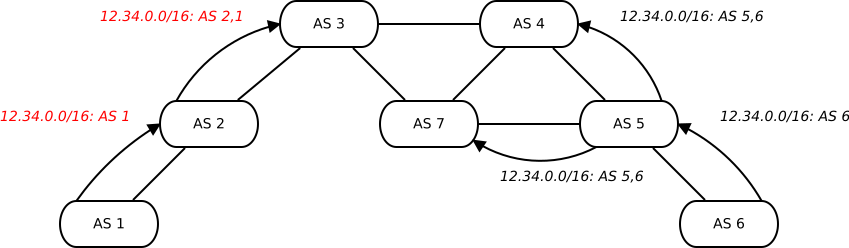
\includegraphics[width=\textwidth]{pathlength.pdf}
				\caption{\textsc{Prefix hijacking by shorter AS pathes}}
			\end{center}
			\label{shortpath}
		\end{figure*}
		Figure \ref{shortpath} shows an example where both AS 1 and AS 6 advertise the prefix 12.34.0.0/16 but just AS 6 owns those prefixes. The autonomous systems 2 and 3 may believe the advertisements from AS 1 because of the shorter path length in comparison to AS 6.

		\paragraph{Deaggregation}
		Another possibility to hijack prefixes is to advertise more specific routes. That means that an IP router would rather prefer a route to a smaller subnet than to a big block of adresses. This behaviour is called \emph{deaggregation.} 
		
		%TODO In 1997  
		\begin{figure*}[ht!]
			\begin{center}
				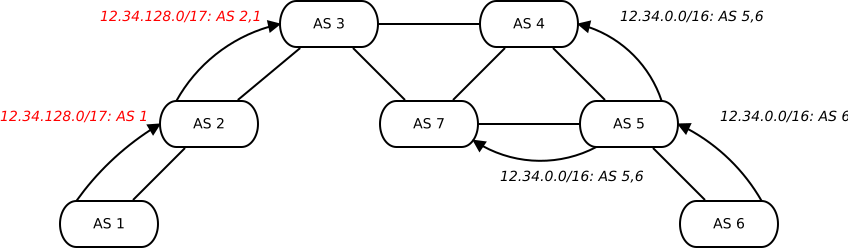
\includegraphics[scale=0.5]{deaggregation.pdf}
				\caption{\textsc{Prefix hijacking by deaggregation}}
			\end{center}
			\label{deaggregation}
		\end{figure*}
		An example of deaggreation is shown in \mbox{Figure \ref{deaggregation}}. Here all other autonomous systems will relay the traffic with destination 12.34.128.0/17 to AS 1, because it anounces a more specific prefix than AS 6 which advertises a larger block of IP addresses (12.34.0.0/16).
		
	       	\subsubsection{Attacks on TCP}
		BGP routers exchange information by utilizing the Transmission Control Protocll (TCP) to construct a realiable, connection-oriented channel between each other. 
		TCP already offers features like retransmission, error correction, congestion and flow control. 
		Since TCP itself does not offer a security mechanism that protects the messages confidentiality and integrity, those threats obviously exist for the communication between BGP routers. 
		In all described techniques we consider two BGP routers named Alice and Bob. The attacker, from now on called Malice, will try to compromise the normal operation and communication of those two routers.

		Possible attacks are eavesdropping on messages to learn routing information or reveal confidential buisness relationsships.
		Additionally, Man In The Middle attacks on TCP allow Malice to insert, modify and delete messages. 
		Also packets could be replayed to withdraw valid routes or re-install already withdrawn routes.
	
		Another way to affect BGP via TCP is a \emph{Denial-of-Service} attack which will leave a BGP router unavailable to its users.
		It can be accomplished by the use of various techniques that will be described here briefly:
		\paragraph{TCP RST}
		A TCP connection can be closed by sending a TCP packet with either the FIN or RST flag set. 
		Malice could disrupt the conversation of Alice and Bob by sending a RST packet which will close the TCP connection between them. TCP has limited protection aka sequence numbers against this method. 

		\paragraph{SYN-Flood}
		The establishment of a TCP connection is initiated with the so called three-way handshake, a sequence of TCP messages with specific flags set. It starts with a SYN packet from Alice. Bob answers this SYN with a SYN-ACK. The handshake is completed by Alice, acknowledging the SYN-ACK from Bob with an ACK.
		Since Bob has to allocate resources when receiving a SYN from Alice, Malice could abuse this and exhaust the resources of Bob by sending alot of SYN packets without completing the handshake. This will make Bob unable to answer any further, real TCP connections. This can also lead to \emph{route flapping} which is described in the next paragraph.
		\paragraph{Route Flapping}
		Route flapping occurs when a router alternatly announces a route as unavailable and available again. When Malice achieves that Bob is no longer availablewith help of a DoS attack, Bobs neighbours will withdraw all routes they learned from Bob. Coming back online, Bob will advertise the routes again to all his neighbours.
		This behaviour results in a high use of network bandwith in addition to the DoS attack. 

		\subsubsection{Attack on the routing policy} 
		
		These attacks aim to influence the routers decision which route out of a set of routes should be chosen for a specific prefix. This decision depends on the attribute values in UPDATE messages. Routing policies of an AS determine on how those values are set and interpreted. The following attributes are considered when chosing a route:
		\begin{itemize}
			\item The local preference attribute is used to prefer specific policies like contracts with customers over shortest-path routing.
			\item The AS path length is considered when multiple routes have the same local preference. The shortest path is chosen.
			\item The Origin type determines where the route was learned from. This could be from inside or outside the AS or from another type of source.
			\item It can occur that two huge have more than peering routers to each other. The MED, Multi-Exit Discriminator determines to which of those locations the data is routed to. 
		\end{itemize}
		By tampering around those attributes the route selection by an AS can be manipulated. 
		For example an AS could simply shorten the AS path length by deleting a few BGP hops in the path.

		%TODO examples?
       \section{BGP security today}
		The target of BGP security research is to reach \emph{Byzantine robustness} of the protocol. That means that all non faulty hosts reach the same descision (agreement) in a finite time period (termination), even if there arey hosts that show faulty behaviour. %cite
		
		Current deployed solutions cannot or just partly fulfill those requirements. They focus on the protection of the underlying TCP connection, try to defensively BGP messages and atempt to setup so called routing registries. In practise, some of them improve the security of BGP but they cannot defend the system against more complex attacks. The next section describes the currently used techniques and what can actually be achieved by them. 



%Cryptographig techniques: 
%	Pairwise keying
%	Cryptographic hash functions
%	MACs
%	Diffie-Hellmann%	PKI
%	Certificates	
	\subsection{Protection of a BGP Session between routers}
		The methods that are used to protect the communication between two BGP speaking routers aim basically in protecting the underlying layers and improving BGP session security.

		\paragraph{MD5 integrity} One proposal to increase the security of BGP is to utilize a TCP extension that uses a message authentication code based on MD5, a message digst algorithm. The extension would include a digest of the TCP header and the BGP message.  This protects the integrity of a TCP packet and thus also prevents replay attacks due to the included protection of TCPs sequence numbers. 
		From performance view MD5 is a very cheap algorithm which is  not computational intensive but from security view MD5 is no longer considered as a secure message digest. %cite

		\paragraph{Session and Message Protection}
		The security of a BGP session can be improved by the following countermeasures, proposed by %TODO cite
		First of all, encrypting BGP data with a secret shared key ensures the confidentiality of the data. 
		Also sequence numbers are proposed to prevent replay attacks and assures the correct order of the packets. Those sequence numbers are somehow 'authenticated' due to the prior encryption. 

		Additionally, it is proposed that the BGP UPDATE messages are equiped with sequence numbers or timestamps.
		Also, a new path attribute, PREDECESSOR is added to an UPDATE message. This would allow the identification of last AS before the destination AS. All of those methods would somehow offer confidentiallity and integrity. The disadvantages are that for this approach BGP needs to be altered. This will make those changes hard to deploy in a large scale. Another drawback is that the encryption is based on shared secrets. The consequence is that for each pair of routers a shared key has to be managed by the administrators which increases the administrative overhead alot.
					       

		\paragraph{Generalized TTL Security Mechanism}
		Generalized TTL Security Mechanism (GTSM) tilizes the IP header field \emph{Time to live} that determines how many hops an IP packet will be valid before it will be dropped by a router. The idea behind this method is to just accept packets with a TTL value greater or equal the value of the maximum TTL minus one. In practise the maximum IP TTL can be 255. A packet with a TTL smaller than 254 would be dropped or may trigger a security alert. This assures that every packet originates just one hop away from the router and defends against remote attackers. The procudure does not protect against malicious information in BGP messages coming from adjacent peers. It is also less usefull in multihop environments, although it could be installed in such. For example, one BGP router could accept packets with a source three hops away. This would also allow attackers to undermine this countermeasure if they are up to three hops away. Also it is possible to encapsulate one IP packet with the maximum TTL set in another IP packet with a destination in the range of the accepted maximum hops. GTSM is a simple and cheap defense but less effective against more sophisticated attacks. 
	
		\paragraph{IPsec}	
		One common approach to secure peer communications is IPsec. IPsec offers security on the network layer, making it transparent to all the overlying applications. It is a protocol that encompasses three areas: authentication, confidentiality and key management. Next to those areas IPsec also offers a mechanism to prevent replay attacks in addition to a weak defense against DoS attacks.

		Three protocols are used to provide security: \emph{Authentication Header} (AH), an extension header to provide authentication and \emph{Encapsulating Security Payload} (ESP) that also encrypts next to its authentication ability. Due to the fact, that ESP offers authentication and encryption, AH is deprecated and should not longer be used in new applications. 
		
		The third protocol called \emph{Internet Key Exchange} (IKE) is responsible for the determination and the distribution of secret keys, which could happen either manually or with an automatic on-demand protocol.

		By using IPsec in the so called tunnel mode the entire original packet is being sent through a virtual tunnel beetween IP endpoints. That means that the payload, the TCP header and the original IP header are encapsulated within an ESP header and trailer and a new IP header is added. This is neccessary due to the encryption of the orginal IP header: No router inbetween could examine the inner IP header. 
		
		So to say, ESP in tunnel mode offers authentication of the ESP header, the original IP header, the TCP header and the payload and also encrypts the entire internet layer data including the ESP trailer. 


		\paragraph{Summary} Summing up, IPsec is a good way to protect a session between peers. It is already widely used but it should become a standard talking about  communication between BGP routers since the more cheap countermeasures like MD5 protection or GTSM are not sufficient enough to prevent intelligent attacks. Table \ref{tab:foo} shows an overview over the described methods and what can be achieved by them.

\begin{table*}[t]
\centering
\begin{tabular}{ l c c c c }
\toprule
                &  Integrity   &  Confidentiality   &  Replay Prevention & DOS Prevention  \\
\midrule
Coutermeasaures  & yes & yes & yes & no \\
GTSM  & no & no & no & no \\
IPsec (AH)  & yes & no & yes & yes \\
IPsec (ESP)  & yes & yes & yes & yes \\
\bottomrule
\end{tabular}
\caption{BGP Peer Session Security Solutions - Requiremnets (Columns) relate to the guarantees provided for AS to AS peering sessions.}%TODO cite
\label{tab:foo}
\end{table*}

       \subsection{Defensive Filtering of suspicious BGP anouncements}

		Another way to improve the security of BGP is to carrefully filter bad and potential malicious announcements.
		Both, ingress and egress filtering is applied based on various route policies.
		First of all, prefixes with special uses like loopback addresses should not be accepted. 
		Also non allocated adresses, address blocks or AS numbers are dropped by routers that use this policy. Those so called bogons can be found in a public list that is kept up to date by the CIDR report. %TODO %cite

		It is also easy to filter private AS numbers. That are numbers given from upstream network providers to customers in order to allow them to communicate with them via BGP without assigning a public AS number to them. Those private AS numbers range from 64512 to 65536.

		In addition it may be useful to drop UPDATE messages that contain a long AS path that exceeds a threshold and routes to small subnets. The latter also prevents global routing tables to be flushed with /24 or smaller address blocks. 
		Moreover a hard limit of announcments a neighbouring AS is permitted to advertise could be set to defend against deaggregation and memory exhaustion of routers.
		Furthermore, an AS could defensivly alter specific BGP attributes before repropagating them. If for example an autonomous system  announces an UPDATE message with the MED attribute and the own policy is to no accept MED values, own routers could rewrite this value in all routes received form that autonomous system.
		
		Summing up, good ingress and egress filtering can improve the security of the own AS as well as the of the  adjacent autonomous systems.
		Filtering is a common and well utilized practise but does not replace a good security architecture because not all autonomous systems seem to filter properly by means of the best practises. If they did, the global routing system would be way more robust against disturbances. 

       \subsection{Routing Registries}
		By being able to build and access a global view on correct routes it is easier to distinguish between valid and malicious/erroneous routes which is so far a very hard task. 
		A global database or registry that would store the prefix and AS ownership, the connectivity between autonomous systems and also the routing policies of each AS. 	
		When building filters a query of a database would allow an AS to just accept routes that are in it. This process is similar to whitelisting.
		
		The requirements of such a registry are accuraty, completeness and security. If attackers could manipulate data in the registry they would be able to cause even more harm if all BGP routers trusted the information stored in it. A global routing registry can be viewed as new single point of failure. 
			
			Also, cooperations would have to publish their routing policy, buisness relationships and topology which is often inadvertent.
			Additionally, it is a hard task to keep a routing registry up to date. Address block allocations change with a high frequency, prefixes are sold, cooperations bust or merge with other cooperations. Those effects of those problems could be reduced by delegating the task of building a routing registry to the authorative registries. In combination with a public key infrastructure, routing registries would offer a good way to provide authenticated information about address and AS number allocations.
		
       \section{BGP Security Solutions}

		All of the so far described solutions are not a sufficient security solution for BGP because they offer just weak cryptographic protection or fail to be able to absolutely determine if a route announcement is bogus or not. Multiple complete, full scale security architectures that provide origin and topology authentication have been proposed. One of those architectures is S-BGP and will be described in the next section.
       \subsection{S-BGP}
		\begin{figure*}[ht!]
			\begin{center}
				\includegraphics[scale=1.337]{sbgp.png}
				\caption{\textsc{Route attestations in S-BGP}}
			\end{center}
			\label{sbgp}
		\end{figure*}
		
			Validates Path attributes in BGP-Update by utilizing a PKI
			Data like adress ownership, peer AS identiy, control messages, policy attributes and path vectors can be digitally signed and verified
			The ownership of a prefix is checked by an out of band mechanism called Adress attestations by the validation of a delegation chain (similar to x509 PKI)
			Route attestations happen within BGP by appending a new attribute to the BGP UPDATE mesage. Each AS in the AS path signs prior signatures.
			Problems: 
				Huge amount of data that needs to be processed and number of possible signers makes this solution computational expensive
				
	\section{Conclusion}				

	
	\section{Literature}

\end{document}
